\documentclass[12pt,twoside,a4paper]{report}
\usepackage[a4paper,width=150mm,top=25mm,bottom=25mm,bindingoffset=6mm]{geometry}

\usepackage[utf8x]{inputenc}
\usepackage[slovak]{babel}
\usepackage{palatino,verbatim}

% Balicek pre priamu rec - \say
\usepackage{dirtytalk}

% Balicek "alltt" je to iste ako "verbatim" mod, ale navyse podporuje aj formatovacie znacky textu
\usepackage{alltt}

% Obrazky
\usepackage{graphicx}
\graphicspath{ {obr/} }

% Cislovanie obrazkov a tabuliek
\usepackage{chngcntr}
%Cisluj obrazky nezavisle od cisla kapitol/podkapitol
\counterwithout{figure}{subsection}
\counterwithout{table}{subsection}

% Referencovanie kapitol/sekcii/... podľa ich nadpisu
\usepackage{nameref}

% Tabulky s viacriadkovymi bunkami a zlucenymi bunkami
% Tabulky generujem naastrojom "http://www.tablesgenerator.com/"
\usepackage{booktabs}
\usepackage{multirow}
% LaTeX ma problemy s prikazmi cline a cmidrule, ked je babel nastaveny na slovencinu/cestinu, kvoli definicii pomlcky
% NAMIESTO POMLCKY POUZI ZNAK ZNAMIENKA MINUS "−" (plati hlavne v nazvoch nadpisov a labelov)
\usepackage{etoolbox}
\preto\tabular{\shorthandoff{-}}

%Uloz obrazok tam, kde je deklarovany
%\usepackage[subsection]{placeins}

\newcommand\sktxt[1]{\foreignlanguage{slovak}{#1}}

\begin{document}
\pagenumbering{arabic}

\setcounter{chapter}{1}
\chapter*{MPLS}
\paragraph{}
Andrej Šišila, Marián Vachalík

\tableofcontents

\newpage
\section{Topológia}
\paragraph{}
Budeme konfigurovať smerovacie protokoly MPLS a IS-IS na topológií, ktorá je znázornená na obrázku \ref{fig:mpls_isis_topo}. V rámci autonómnych systémov sme konfigurovali smerovacie protokoly IS-IS (pokiaľ má autonómny systém viac ako 2 smerovače) a BGP (iBGP). Medzi autonómnymi systémami sme konfigurovali len BGP (eBGP). IP adresácia je uvedená v tabuľke \ref{tab:ip_adresacia} a dopĺňa grafické znázornenie topológie na obrázku \ref{fig:mpls_isis_topo}. Smerovače R6 a R7 sme nekonfigurovali.

\begin{figure}[!htbp]
\centering
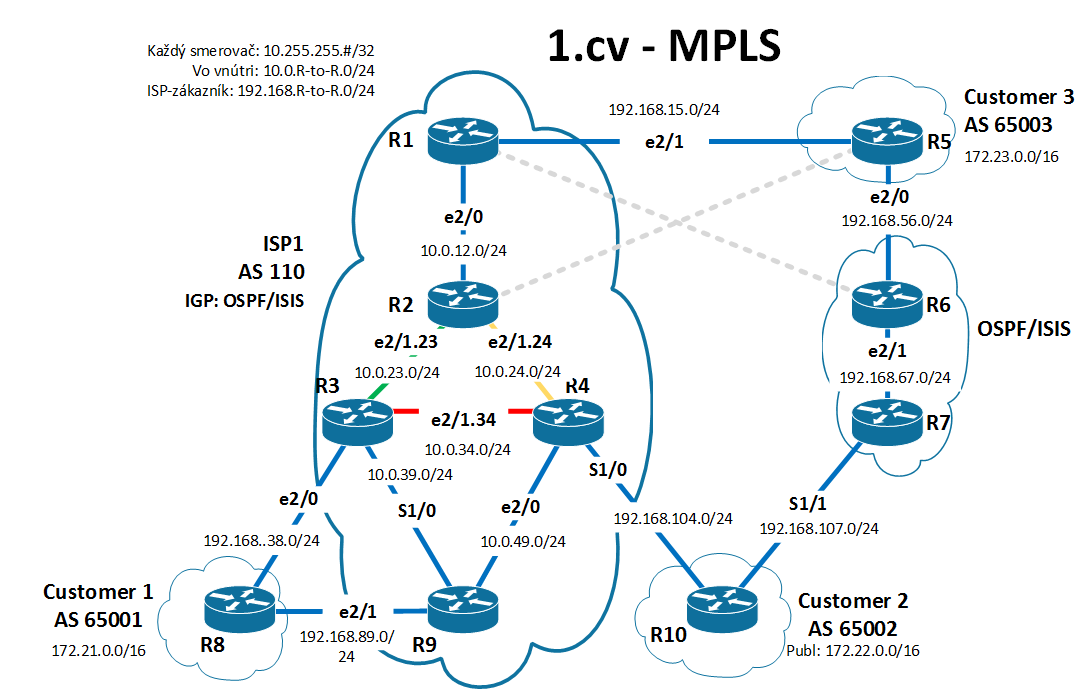
\includegraphics[width=14cm,keepaspectratio]{mpls_isis_topo}
\caption{Topológia MPLS}
\label{fig:mpls_isis_topo}
\end{figure}

\begin{figure}[!htbp]
\centering
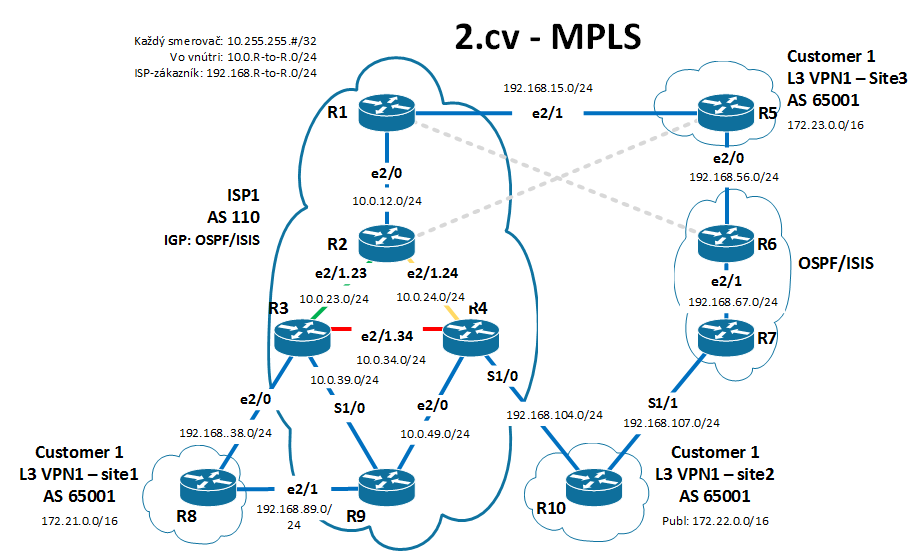
\includegraphics[width=14cm,keepaspectratio]{mpls_l3vpn_topo}
\caption{Topológia MPLS + L3 VPN}
\label{fig:mpls_l3vpn_topo}
\end{figure}



\clearpage


\begin{table}[!htbp]
\centering
\caption{IP adresácia}
\label{tab:ip_adresacia}
\begin{tabular}{|c|l|l|l|}
\hline
\textbf{Smerovač}    & \multicolumn{1}{c|}{\textbf{Rozhranie}} & \multicolumn{1}{c|}{\textbf{IP adresa}} & \multicolumn{1}{c|}{\textbf{Maska}} \\ \hline
\multirow{5}{*}{R1}  & Fa0/0                                   & 200.110.255.249                         & 255.255.255.252                     \\ \cline{2-4} 
                     & Fa0/1                                   & 64.34.255.253                           & 255.255.255.252                     \\ \cline{2-4} 
                     & S1/0                                    & 200.33.255.253                          & 255.255.255.252                     \\ \cline{2-4} 
                     & Lo0                                     & 10.255.255.1                            & 255.255.255.0                       \\ \cline{2-4} 
                     & Lo100                                   & 64.34.1.1                               & 255.255.255.128                     \\ \hline
\multirow{6}{*}{R2}  & Fa0/0                                   & 200.110.255.250                         & 255.255.255.252                     \\ \cline{2-4} 
                     & Fa0/1.23                                & 10.110.23.2                             & 255.255.255.0                       \\ \cline{2-4} 
                     & Fa0/1.24                                & 10.110.24.2                             & 255.255.255.0                       \\ \cline{2-4} 
                     & S1/0                                    & 200.110.255.253                         & 255.255.255.252                     \\ \cline{2-4} 
                     & Lo0                                     & 10.255.255.2                            & 255.255.255.0                       \\ \cline{2-4} 
                     & Lo100                                   & 200.110.0.2                             & 255.255.255.128                     \\ \hline
\multirow{5}{*}{R3}  & Fa0/0                                   & 200.110.255.241                         & 255.255.255.252                     \\ \cline{2-4} 
                     & Fa0/1.23                                & 10.110.23.3                             & 255.255.255.0                       \\ \cline{2-4} 
                     & Fa0/1.34                                & 10.110.34.3                             & 255.255.255.0                       \\ \cline{2-4} 
                     & Lo0                                     & 10.255.255.3                            & 255.255.255.0                       \\ \cline{2-4} 
                     & Lo100                                   & 200.110.0.133                           & 255.255.255.128                     \\ \hline
\multirow{6}{*}{R4}  & Fa0/0                                   & 200.110.255.237                         & 255.255.255.252                     \\ \cline{2-4} 
                     & Fa0/1.24                                & 10.110.24.4                             & 255.255.255.0                       \\ \cline{2-4} 
                     & Fa0/1.34                                & 10.110.34.4                             & 255.255.255.0                       \\ \cline{2-4} 
                     & S1/0                                    & 200.110.255.245                         & 255.255.255.252                     \\ \cline{2-4} 
                     & Lo0                                     & 10.255.255.4                            & 255.255.255.0                       \\ \cline{2-4} 
                     & Lo100                                   & 200.110.1.4                             & 255.255.255.128                     \\ \hline
\multirow{5}{*}{R5}  & Fa0/0                                   & 200.33.255.249                          & 255.255.255.252                     \\ \cline{2-4} 
                     & Fa0/1                                   & 10.100.15.2                             & 255.255.255.252                     \\ \cline{2-4} 
                     & S1/0                                    & 200.110.255.254                         & 255.255.255.252                     \\ \cline{2-4} 
                     & Lo0                                     & 10.255.255.5                            & 255.255.255.0                       \\ \cline{2-4} 
                     & Lo100                                   & 128.45.5.5                              & 255.255.255.128                     \\ \hline
\multirow{5}{*}{R6}  & Fa0/0                                   & 200.33.255.250                          & 255.255.255.252                     \\ \cline{2-4} 
                     & Fa0/1                                   & 10.110.67.6                             & 255.255.255.0                       \\ \cline{2-4} 
                     & S1/0                                    & 200.33.255.254                          & 255.255.255.252                     \\ \cline{2-4} 
                     & Lo0                                     & 10.255.255.6                            & 255.255.255.0                       \\ \cline{2-4} 
                     & Lo100                                   & 200.33.6.6                              & 255.255.255.128                     \\ \hline
\multirow{4}{*}{R7}  & Fa0/1                                   & 10.110.67.7                             & 255.255.255.0                       \\ \cline{2-4} 
                     & S1/1                                    & 200.33.255.245                          & 255.255.255.252                     \\ \cline{2-4} 
                     & Lo0                                     & 10.255.255.7                            & 255.255.255.0                       \\ \cline{2-4} 
                     & Lo100                                   & 200.33.7.7                              & 255.255.255.128                     \\ \hline
\multirow{4}{*}{R8}  & Fa0/0                                   & 200.110.255.242                         & 255.255.255.252                     \\ \cline{2-4} 
                     & Fa0/1                                   & 10.110.89.8                             & 255.255.255.0                       \\ \cline{2-4} 
                     & Lo0                                     & 10.255.255.8                            & 255.255.255.0                       \\ \cline{2-4} 
                     & Lo100                                   & 200.110.12.8                            & 255.255.255.128                     \\ \hline
\multirow{4}{*}{R9}  & Fa0/0                                   & 200.110.255.238                         & 255.255.255.252                     \\ \cline{2-4} 
                     & Fa0/1                                   & 10.110.89.9                             & 255.255.255.0                       \\ \cline{2-4} 
                     & Lo0                                     & 10.255.255.9                            & 255.255.255.0                       \\ \cline{2-4} 
                     & Lo100                                   & 200.110.13.9                            & 255.255.255.128                     \\ \hline
\multirow{4}{*}{R10} & S1/0                                    & 200.110.255.246                         & 255.255.255.252                     \\ \cline{2-4} 
                     & S1/1                                    & 200.33.255.246                          & 255.255.255.252                     \\ \cline{2-4} 
                     & Lo0                                     & 10.255.255.10                           & 255.255.255.0                       \\ \cline{2-4} 
                     & Lo100                                   & 223.255.255.10                          & 255.255.255.128                     \\ \hline
\end{tabular}
\end{table}


% Novu kapitolu davam na novu stranu, lebo bez toho mi zobrazuje tabulku v dalsej kapitole, kde ale tabulka nepatri.
\clearpage

\section{Úlohy}
\subsection{IS−IS alebo OSPF}
\subsubsection{Popis}
\paragraph{}
Ako vnútorný protokol sme zvolili IS-IS. Jeho konfigurácia je rovnaká ako v predchádzajúcich cvičeniach s ohľadom na aktuálny adresný plán.

\subsubsection{Konfigurácia}
\paragraph{}
IS-IS sme konfigurovali na R1, R2, R3, R4 a R9

\noindent
{\fontfamily{qcr}\selectfont
\begin{small}
\begin{alltt}
R1(config)#router isis
  net 49.0002.0102.5525.5001.00
  exit
int e2/0
  ip router isis
  isis network point-to-point
int lo0
  ip router isis
\end{alltt}
\end{small}
}

\subsubsection{Overenie}
\paragraph{}
Konfiguráciu IS-IS sme overovali zobrazením IS-IS databázy.

\noindent
{\fontfamily{qcr}\selectfont
\begin{small}
\begin{alltt}
R1# show isis database
\end{alltt}
\end{small}
}







\subsection{MPLS}
\subsubsection{Popis}
\paragraph{}
Základnú konfiguráciu MPLS sme robili podľa stránky \say{nil.uniza.sk}. Najprv zapneme \say{Cisco express forwarding} príkazom \say{ip cef}. Potom aktivujeme LDP značkovanie príkazom \say{mpls label protocol ldp}. Nakoniec zapneme MPLS príkazom \say{mpls ip}. Príkaz \say{mpls ip} sme použili iba na rozhraniach vnútri providerskej siete, nie na PE smerovačoch smerom k zákazníkom.

\subsubsection{Konfigurácia}
\paragraph{}
Aby sme zabezpečili konektivitu medzi jednotlivými zákazníkmi R5, R8 a R10, je potrebné nakonfigurovať BGP medzi týmito smerovačmi a ich susedmi v ISP1. Rovnako aj ohlasujeme požadovanú sieť zákazníka, v našom prípade Lo0. Na smerovači R2 BGP nekonfigurujeme.

\noindent
{\fontfamily{qcr}\selectfont
\begin{small}
\begin{alltt}
R1 (config)#ip cef
mpls ip
mpls label protocol ldp
int serial1/0
  mpls ip
router bgp 65003
  neighbor 192.168.15.1 remote-as 110
  address-family ipv4 unicast
  neighbor 192.168.15.1 activate
  network 10.255.255.5 mask 255.255.255.255
\end{alltt}
\end{small}
}

\subsubsection{Overenie}
\paragraph{}
\noindent
{\fontfamily{qcr}\selectfont
\begin{small}
\begin{alltt}
show mpls ldp discovery
sh ip bgp ipv4 unicast
traceroute 10.255.255.8 source l0 =\textgreater sledovat znacku
\end{alltt}
\end{small}
}






\subsection{LDP alebo RSVP}
\subsubsection{Popis}
\paragraph{}

\subsubsection{Konfigurácia}
\paragraph{}

\subsubsection{Overenie}
\paragraph{}






\subsection{Router Reflector alebo konfederácie}
\subsubsection{Popis}
\paragraph{}
V tomto prípade sme sa dohodli o nastavení Route Reflectora (RR) na smerovač R1. RR je BGP smerovač, ktorý obchádza pravidlo, že iBGP topológia musí byť \say{full-mesh} t.j. iBGP smerovač v jednej oblasti nešíri prefixy, ktoré sa naučil cez iBGP smerovač z inej oblasti.



\subsubsection{Konfigurácia}
\paragraph{}
Smerovače R3, R4 a R9 sme nastavovali ako museli nadviazať BGP s R1.

\noindent
{\fontfamily{qcr}\selectfont
\begin{small}
\begin{alltt}
router bgp 110
  neighbor 10.255.255.1 remote-as 110
  neighbor 10.255.255.1 update-source Loopback0
  address-family ipv4 unicast
    neighbor 10.255.255.1 activate
    neighbor 10.255.255.1 next-hop-self
  network 10.255.255.3 mask 255.255.255.255
\end{alltt}
\end{small}
}

\paragraph{}
Potom nasledovala konfigurácia RR, teda smerovača R1.

\noindent
{\fontfamily{qcr}\selectfont
\begin{small}
\begin{alltt}
R1
router bgp 110
  neighbor 10.255.255.3 remote-as 110
  neighbor 10.255.255.3 update-source l0
  neighbor 10.255.255.4 remote-as 110
  neighbor 10.255.255.4 update-source l0
  neighbor 10.255.255.9 remote-as 110
  neighbor 10.255.255.9 update-source l0
  address-family ipv4 unicast
    neighbor 10.255.255.3 route-reflector-client
    neighbor 10.255.255.3 send-community extended
    neighbor 10.255.255.3 next-hop-self
    neighbor 10.255.255.3 activate
    neighbor 10.255.255.4 route-reflector-client
    neighbor 10.255.255.4 send-community extended
    neighbor 10.255.255.4 next-hop-self
    neighbor 10.255.255.4 activate
    neighbor 10.255.255.9 route-reflector-client
    neighbor 10.255.255.9 send-community extended
    neighbor 10.255.255.9 next-hop-self
    neighbor 10.255.255.9 activate 
\end{alltt}
\end{small}
}

\subsubsection{Overenie}
\paragraph{}
Konektivita by mala byť v tomto prípade už všade. Presvedčíme sa pomocou tcl skriptu.

\noindent
{\fontfamily{qcr}\selectfont
\begin{small}
\begin{alltt}
R1#tclsh
R1(tcl)#foreach address {
+>(tcl)#10.255.255.1
+>(tcl)#10.255.255.2
+>(tcl)#10.255.255.3
+>(tcl)#10.255.255.4
+>(tcl)#10.255.255.5
+>(tcl)#10.255.255.6
+>(tcl)#10.255.255.7
+>(tcl)#10.255.255.8
+>(tcl)#10.255.255.9
+>(tcl)#10.255.255.10
+>(tcl)#} {
+>(tcl)#ping $address source 10.255.255.1}
Sending 5, 100-byte ICMP Echos to 10.255.255.1, timeout is 2 seconds:
!!!!!
Success rate is 100 percent (5/5), round-trip min/avg/max = 8/8/8 ms
Sending 5, 100-byte ICMP Echos to 10.255.255.2, timeout is 2 seconds:
!!!!!
Success rate is 100 percent (5/5), round-trip min/avg/max = 16/22/28 ms
Sending 5, 100-byte ICMP Echos to 10.255.255.3, timeout is 2 seconds:
!!!!!
Success rate is 100 percent (5/5), round-trip min/avg/max = 24/39/68 ms
Sending 5, 100-byte ICMP Echos to 10.255.255.4, timeout is 2 seconds:
!!!!!
Success rate is 100 percent (5/5), round-trip min/avg/max = 16/33/52 ms
Sending 5, 100-byte ICMP Echos to 10.255.255.5, timeout is 2 seconds:
!!!!!
Success rate is 100 percent (5/5), round-trip min/avg/max = 16/26/40 ms
Sending 5, 100-byte ICMP Echos to 10.255.255.8, timeout is 2 seconds:
!!!!!
Success rate is 100 percent (5/5), round-trip min/avg/max = 72/88/100 ms
Sending 5, 100-byte ICMP Echos to 10.255.255.9, timeout is 2 seconds:
!!!!!
Success rate is 100 percent (5/5), round-trip min/avg/max = 48/63/80 ms
Sending 5, 100-byte ICMP Echos to 10.255.255.10, timeout is 2 seconds:
!!!!!
Success rate is 100 percent (5/5), round-trip min/avg/max = 72/79/100 ms
\end{alltt}
\end{small}
}

TODO - ZLE - nejak tam treba zakomponovat tie RED GREEN - urobit cez VRF PING








\subsection{Multiprotocol BGP}
\subsubsection{Popis}
\paragraph{}

\subsubsection{Konfigurácia}
\paragraph{}

\noindent
{\fontfamily{qcr}\selectfont
\begin{small}
\begin{alltt}
R1(config)#do sh run
Building configuration...

Current configuration : 3764 bytes
!
! Last configuration change at 09:05:48 UTC Tue May 9 2017
upgrade fpd auto
version 15.3
service timestamps debug datetime msec
service timestamps log datetime msec
no service password-encryption
!
hostname R1
!
boot-start-marker
boot-end-marker
!
aqm-register-fnf
!
!
no aaa new-model
!
!
!
ip vrf GREEN
 rd 100:2 
 route-target export 110:2
 route-target import 110:2
!
ip vrf RED
 rd 110:1
 route-target export 110:1
 route-target import 110:1
!
!
!
!
no ip domain lookup
ip cef
no ipv6 cef
!
multilink bundle-name authenticated
mpls label protocol ldp
!
!
!
!
!
!         
!
!
!
username admin privilege 15 secret 5 $1$eKi3$TJSJS.zu5o6JMF5F3h4bV1
!
redundancy
!
!
! 
!
!
!
!
!
!
!
!
!
interface Loopback0
 ip address 10.255.255.1 255.255.255.255
 ip router isis 
!
interface Loopback1
 ip vrf forwarding GREEN
 ip address 172.23.0.1 255.255.0.0
!
interface FastEthernet0/0
 no ip address
 shutdown
 duplex half
!
interface Serial1/0
 no ip address
 shutdown
 serial restart-delay 0
!
interface Serial1/1
 no ip address
 shutdown
 serial restart-delay 0
!
interface Serial1/2
 no ip address
 shutdown
 serial restart-delay 0
!         
interface Serial1/3
 no ip address
 shutdown
 serial restart-delay 0
!
interface Serial1/4
 no ip address
 shutdown
 serial restart-delay 0
!
interface Serial1/5
 no ip address
 shutdown
 serial restart-delay 0
!
interface Serial1/6
 no ip address
 shutdown
 serial restart-delay 0
!
interface Serial1/7
 no ip address
 shutdown 
 serial restart-delay 0
!
interface Ethernet2/0
 ip address 10.0.12.1 255.255.255.0
 ip router isis 
 duplex half
 mpls ip
 isis network point-to-point 
!
interface Ethernet2/1
 ip vrf forwarding RED
 ip address 192.168.15.1 255.255.255.0
 duplex half
!
interface Ethernet2/2
 no ip address
 shutdown
 duplex half
!
interface Ethernet2/3
 no ip address
 shutdown
 duplex half
!
interface Ethernet2/4
 no ip address
 shutdown
 duplex half
!
interface Ethernet2/5
 no ip address
 shutdown
 duplex half
!
interface Ethernet2/6
 no ip address
 shutdown
 duplex half
!
interface Ethernet2/7
 no ip address
 shutdown
 duplex half
!
router isis
 net 49.0001.0102.5525.5001.00
!
router bgp 110
 bgp log-neighbor-changes
 no bgp default ipv4-unicast
 neighbor 10.255.255.3 remote-as 110
 neighbor 10.255.255.3 update-source Loopback0
 neighbor 10.255.255.4 remote-as 110
 neighbor 10.255.255.4 update-source Loopback0
 neighbor 10.255.255.9 remote-as 110
 neighbor 10.255.255.9 update-source Loopback0
 !
 address-family ipv4
 exit-address-family
 !
 address-family vpnv4
  neighbor 10.255.255.3 activate
  neighbor 10.255.255.3 send-community extended
  neighbor 10.255.255.3 route-reflector-client
  neighbor 10.255.255.4 activate
  neighbor 10.255.255.4 send-community extended
  neighbor 10.255.255.4 route-reflector-client
  neighbor 10.255.255.9 activate
  neighbor 10.255.255.9 send-community extended
  neighbor 10.255.255.9 route-reflector-client
 exit-address-family
 !
 address-family ipv4 vrf GREEN
  redistribute connected
 exit-address-family
 !
 address-family ipv4 vrf RED
  redistribute connected
  neighbor 192.168.15.5 remote-as 65001
  neighbor 192.168.15.5 activate
  neighbor 192.168.15.5 as-override
 exit-address-family
!
ip forward-protocol nd
no ip http server
no ip http secure-server
!
!
!
!
!
mpls ldp router-id Loopback0 force
!
control-plane
!
!
mgcp behavior rsip-range tgcp-only
mgcp behavior comedia-role none
mgcp behavior comedia-check-media-src disable
mgcp behavior comedia-sdp-force disable
!
mgcp profile default
!
!
!
gatekeeper
 shutdown
!
!
line con 0
 exec-timeout 120 0
 logging synchronous
 login local
 stopbits 1
line aux 0
 stopbits 1
line vty 0 4
 privilege level 15
 no login
 transport input all
line vty 5 15
 privilege level 15
 no login
 transport input all
!
!
end

R1(config)# 
==================
R2(config-subif)#do sh run
Building configuration...

Current configuration : 2739 bytes
!
! Last configuration change at 09:06:53 UTC Tue May 9 2017
upgrade fpd auto
version 15.3
service timestamps debug datetime msec
service timestamps log datetime msec
no service password-encryption
!
hostname R2
!
boot-start-marker
boot-end-marker
!
aqm-register-fnf
!
!
no aaa new-model
!
!
!
!
!         
!
no ip domain lookup
ip cef
no ipv6 cef
!
multilink bundle-name authenticated
mpls label protocol ldp
!
!
!
!
!
!
!
!
!
username admin privilege 15 secret 5 $1$QNaa$DSiUgQZG.ZRbem2tUy4nv.
!
redundancy
!
!
! 
!         
!
!
!
!
!
!
!
!
interface Loopback0
 ip address 10.255.255.2 255.255.255.255
 ip router isis 
!
interface FastEthernet0/0
 no ip address
 shutdown
 duplex half
!
interface Serial1/0
 no ip address
 shutdown
 serial restart-delay 0
!
interface Serial1/1
 no ip address
 shutdown
 serial restart-delay 0
!
interface Serial1/2
 no ip address
 shutdown
 serial restart-delay 0
!
interface Serial1/3
 no ip address
 shutdown
 serial restart-delay 0
!
interface Serial1/4
 no ip address
 shutdown
 serial restart-delay 0
!
interface Serial1/5
 no ip address
 shutdown
 serial restart-delay 0
!
interface Serial1/6
 no ip address
 shutdown
 serial restart-delay 0
!
interface Serial1/7
 no ip address
 shutdown
 serial restart-delay 0
!
interface Ethernet2/0
 ip address 10.0.12.2 255.255.255.0
 ip router isis 
 duplex half
 mpls ip
 isis network point-to-point 
!
interface Ethernet2/1
 no ip address
 shutdown
 duplex half
 isis network point-to-point 
!
interface Ethernet2/1.23
 encapsulation dot1Q 23
 ip address 10.0.23.2 255.255.255.0
 ip router isis 
 mpls ip
 isis network point-to-point 
!
interface Ethernet2/1.24
 encapsulation dot1Q 24
 ip address 10.0.24.2 255.255.255.0
 ip router isis 
 mpls ip
 isis network point-to-point 
!
interface Ethernet2/2
 no ip address
 shutdown
 duplex half
!
interface Ethernet2/3
 no ip address
 shutdown 
 duplex half
!
interface Ethernet2/4
 no ip address
 shutdown
 duplex half
!
interface Ethernet2/5
 no ip address
 shutdown
 duplex half
!
interface Ethernet2/6
 no ip address
 shutdown
 duplex half
!
interface Ethernet2/7
 no ip address
 shutdown
 duplex half
!
router isis
 net 49.0001.0102.5525.5002.00
!
ip forward-protocol nd
no ip http server
no ip http secure-server
!
!
!
!
!
mpls ldp router-id Loopback0 force
!
control-plane
!
!
mgcp behavior rsip-range tgcp-only
mgcp behavior comedia-role none
mgcp behavior comedia-check-media-src disable
mgcp behavior comedia-sdp-force disable
!
mgcp profile default
!
!         
!
gatekeeper
 shutdown
!
!
line con 0
 exec-timeout 120 0
 logging synchronous
 login local
 stopbits 1
line aux 0
 stopbits 1
line vty 0 4
 privilege level 15
 no login
 transport input all
line vty 5 15
 privilege level 15
 no login
 transport input all
!
!
end       

R2(config-subif)#   
============================
R3(config)#do sh run
Building configuration...

Current configuration : 3254 bytes
!
! Last configuration change at 09:08:12 UTC Tue May 9 2017
upgrade fpd auto
version 15.3
service timestamps debug datetime msec
service timestamps log datetime msec
no service password-encryption
!
hostname R3
!
boot-start-marker
boot-end-marker
!
aqm-register-fnf
!
!
no aaa new-model
!
!
!
ip vrf RED
 rd 110:1 
 route-target export 110:1
 route-target import 110:1
!
!
!
!
no ip domain lookup
ip cef
no ipv6 cef
!
multilink bundle-name authenticated
mpls label protocol ldp
!
!
!
!
!
!
!
!
!
username admin privilege 15 secret 5 $1$ierK$7ZnPCJ2hvc7ypP11a//Tc.
!         
redundancy
!
!
! 
!
!
!
!
!
!
!
!
!
interface Loopback0
 ip address 10.255.255.3 255.255.255.255
 ip router isis 
!
interface FastEthernet0/0
 no ip address
 shutdown
 duplex half
!
interface Serial1/0
 ip address 10.0.39.3 255.255.255.0
 ip router isis 
 mpls ip
 serial restart-delay 0
!
interface Serial1/1
 no ip address
 shutdown
 serial restart-delay 0
!
interface Serial1/2
 no ip address
 shutdown
 serial restart-delay 0
!
interface Serial1/3
 no ip address
 shutdown
 serial restart-delay 0
!
interface Serial1/4
 no ip address
 shutdown 
 serial restart-delay 0
!
interface Serial1/5
 no ip address
 shutdown
 serial restart-delay 0
!
interface Serial1/6
 no ip address
 shutdown
 serial restart-delay 0
!
interface Serial1/7
 no ip address
 shutdown
 serial restart-delay 0
!
interface Ethernet2/0
 ip vrf forwarding RED
 ip address 192.168.38.3 255.255.255.0
 duplex half
!
interface Ethernet2/1
 no ip address
 duplex half
 isis network point-to-point 
!
interface Ethernet2/1.23
 encapsulation dot1Q 23
 ip address 10.0.23.3 255.255.255.0
 ip router isis 
 mpls ip
 isis network point-to-point 
!
interface Ethernet2/1.34
 encapsulation dot1Q 34
 ip address 10.0.34.3 255.255.255.0
 ip router isis 
 mpls ip
 isis network point-to-point 
!
interface Ethernet2/2
 no ip address
 shutdown
 duplex half
!         
interface Ethernet2/3
 no ip address
 shutdown
 duplex half
!
interface Ethernet2/4
 no ip address
 shutdown
 duplex half
!
interface Ethernet2/5
 no ip address
 shutdown
 duplex half
!
interface Ethernet2/6
 no ip address
 shutdown
 duplex half
!
interface Ethernet2/7
 no ip address
 shutdown 
 duplex half
!
router isis
 net 49.0001.0102.5525.5003.00
!
router bgp 110
 bgp log-neighbor-changes
 neighbor 10.255.255.1 remote-as 110
 neighbor 10.255.255.1 update-source Loopback0
 !
 address-family vpnv4
  neighbor 10.255.255.1 activate
  neighbor 10.255.255.1 send-community extended
 exit-address-family
 !
 address-family ipv4 vrf RED
  redistribute connected
  neighbor 192.168.38.8 remote-as 65001
  neighbor 192.168.38.8 activate
  neighbor 192.168.38.8 as-override
 exit-address-family
!
ip forward-protocol nd
no ip http server
no ip http secure-server
!
!
!
!
!
mpls ldp router-id Loopback0 force
!
control-plane
!
!
mgcp behavior rsip-range tgcp-only
mgcp behavior comedia-role none
mgcp behavior comedia-check-media-src disable
mgcp behavior comedia-sdp-force disable
!
mgcp profile default
!
!
!
gatekeeper
 shutdown 
!
!
line con 0
 exec-timeout 120 0
 logging synchronous
 login local
 stopbits 1
line aux 0
 stopbits 1
line vty 0 4
 privilege level 15
 no login
 transport input all
line vty 5 15
 privilege level 15
 no login
 transport input all
!
!
end

=-==================
R4(config)#
*May  9 09:46:52.772: %LDP-5-NBRCHG: LDP Neighbor 10.255.255.3:0 (1) is UP
R4(config)#do sh run
Building configuration...

Current configuration : 3599 bytes
!
! Last configuration change at 09:09:38 UTC Tue May 9 2017
upgrade fpd auto
version 15.3
service timestamps debug datetime msec
service timestamps log datetime msec
no service password-encryption
!
hostname R4
!
boot-start-marker
boot-end-marker
!
aqm-register-fnf
!
!
no aaa new-model
!
!
!
ip vrf GREEN
 rd 110:2 
 route-target export 110:2
 route-target import 110:2
!
ip vrf RED
 rd 110:1
 route-target export 110:1
 route-target import 110:1
!
!
!
!
no ip domain lookup
ip cef
no ipv6 cef
!
multilink bundle-name authenticated
mpls label protocol ldp
!
!
!
!
!
!         
!
!
!
username admin privilege 15 secret 5 $1$Eu2a$rgRjxOvteTJdNyTEKValI/
!
redundancy
!
!
! 
!
!
!
!
!
!
!
!
!
interface Loopback0
 ip address 10.255.255.4 255.255.255.255
 ip router isis 
!
interface Loopback1
 ip vrf forwarding GREEN
 ip address 172.22.0.1 255.255.0.0
!
interface FastEthernet0/0
 no ip address
 shutdown
 duplex half
!
interface Serial1/0
 ip vrf forwarding RED
 ip address 192.168.104.4 255.255.255.0
 serial restart-delay 0
!
interface Serial1/1
 no ip address
 shutdown
 serial restart-delay 0
!
interface Serial1/2
 no ip address
 shutdown
 serial restart-delay 0
!         
interface Serial1/3
 no ip address
 shutdown
 serial restart-delay 0
!
interface Serial1/4
 no ip address
 shutdown
 serial restart-delay 0
!
interface Serial1/5
 no ip address
 shutdown
 serial restart-delay 0
!
interface Serial1/6
 no ip address
 shutdown
 serial restart-delay 0
!
interface Serial1/7
 no ip address
 shutdown 
 serial restart-delay 0
!
interface Ethernet2/0
 ip address 10.0.49.4 255.255.255.0
 ip router isis
 duplex half
 mpls ip
 isis network point-to-point 
!
interface Ethernet2/1
 no ip address
 duplex half
 isis network point-to-point 
!
interface Ethernet2/1.23
 isis network point-to-point 
!
interface Ethernet2/1.24
 encapsulation dot1Q 24
 ip address 10.0.24.4 255.255.255.0
 ip router isis 
 mpls ip  
 isis network point-to-point 
!
interface Ethernet2/1.34
 encapsulation dot1Q 34
 ip address 10.0.34.4 255.255.255.0
 ip router isis 
 mpls ip
 isis network point-to-point 
!
interface Ethernet2/2
 no ip address
 shutdown
 duplex half
!
interface Ethernet2/3
 no ip address
 shutdown
 duplex half
!
interface Ethernet2/4
 no ip address
 shutdown
 duplex half
!
interface Ethernet2/5
 no ip address
 shutdown
 duplex half
!
interface Ethernet2/6
 no ip address
 shutdown
 duplex half
!
interface Ethernet2/7
 no ip address
 shutdown
 duplex half
!
router isis
 net 49.0001.0102.5525.5004.00
!
router bgp 110
 bgp log-neighbor-changes
 neighbor 10.255.255.1 remote-as 110
 neighbor 10.255.255.1 update-source Loopback0
 !
 address-family vpnv4
  neighbor 10.255.255.1 activate
  neighbor 10.255.255.1 send-community extended
 exit-address-family
 !
 address-family ipv4 vrf GREEN
  redistribute connected
 exit-address-family
 !
 address-family ipv4 vrf RED
  redistribute connected
  neighbor 192.168.104.10 remote-as 65001
  neighbor 192.168.104.10 activate
  neighbor 192.168.104.10 as-override
 exit-address-family
!
ip forward-protocol nd
no ip http server
no ip http secure-server
!
!
!         
!
!
mpls ldp router-id Loopback0 force
!
control-plane
!
!
mgcp behavior rsip-range tgcp-only
mgcp behavior comedia-role none
mgcp behavior comedia-check-media-src disable
mgcp behavior comedia-sdp-force disable
!
mgcp profile default
!
!
!
gatekeeper
 shutdown
!
!
line con 0
 exec-timeout 120 0
 logging synchronous
 login local
 stopbits 1
line aux 0
 stopbits 1
line vty 0 4
 privilege level 15
 no login
 transport input all
line vty 5 15
 privilege level 15
 no login
 transport input all
!
!
end

==================
R5(config)#do sh run
Building configuration...

Current configuration : 2432 bytes
!
! Last configuration change at 09:10:04 UTC Tue May 9 2017
upgrade fpd auto
version 15.3
service timestamps debug datetime msec
service timestamps log datetime msec
no service password-encryption
!
hostname R5
!
boot-start-marker
boot-end-marker
!
aqm-register-fnf
!
!
no aaa new-model
!
!
!
!
!         
!
no ip domain lookup
ip cef
no ipv6 cef
!
multilink bundle-name authenticated
!
!
!
!
!
!
!
!
!
username admin privilege 15 secret 5 $1$n4c4$fjx3bLiFEXqL3tjOX2tda/
!
redundancy
!
!
! 
!
!         
!
!
!
!
!
!
!
interface Loopback0
 ip address 10.255.255.5 255.255.255.255
!
interface Loopback1
 ip address 172.23.0.1 255.255.0.0
!
interface FastEthernet0/0
 no ip address
 shutdown
 duplex half
!
interface Serial1/0
 no ip address
 shutdown
 serial restart-delay 0
!         
interface Serial1/1
 no ip address
 shutdown
 serial restart-delay 0
!
interface Serial1/2
 no ip address
 shutdown
 serial restart-delay 0
!
interface Serial1/3
 no ip address
 shutdown
 serial restart-delay 0
!
interface Serial1/4
 no ip address
 shutdown
 serial restart-delay 0
!
interface Serial1/5
 no ip address
 shutdown 
 serial restart-delay 0
!
interface Serial1/6
 no ip address
 shutdown
 serial restart-delay 0
!
interface Serial1/7
 no ip address
 shutdown
 serial restart-delay 0
!
interface Ethernet2/0
 no ip address
 shutdown
 duplex half
!
interface Ethernet2/1
 ip address 192.168.15.5 255.255.255.0
 duplex half
!
interface Ethernet2/2
 no ip address
 shutdown
 duplex half
!
interface Ethernet2/3
 no ip address
 shutdown
 duplex half
!
interface Ethernet2/4
 no ip address
 shutdown
 duplex half
!
interface Ethernet2/5
 no ip address
 shutdown
 duplex half
!
interface Ethernet2/6
 no ip address
 shutdown
 duplex half
!         
interface Ethernet2/7
 no ip address
 shutdown
 duplex half
!
router bgp 65001
 bgp log-neighbor-changes
 network 172.23.0.0
 redistribute connected
 neighbor 192.168.15.1 remote-as 110
!
ip forward-protocol nd
no ip http server
no ip http secure-server
!
!
!
!
!
!
control-plane
!
!         
mgcp behavior rsip-range tgcp-only
mgcp behavior comedia-role none
mgcp behavior comedia-check-media-src disable
mgcp behavior comedia-sdp-force disable
!
mgcp profile default
!
!
!
gatekeeper
 shutdown
!
!
line con 0
 exec-timeout 120 0
 logging synchronous
 login local
 stopbits 1
line aux 0
 stopbits 1
line vty 0 4
 privilege level 15
 no login 
 transport input all
line vty 5 15
 privilege level 15
 no login
 transport input all
!
!
end
===============
R8(config-router)#do sh run
Building configuration...

Current configuration : 1943 bytes
!
! Last configuration change at 09:10:47 UTC Tue May 9 2017
upgrade fpd auto
version 15.3
service timestamps debug datetime msec
service timestamps log datetime msec
no service password-encryption
!
hostname R8
!
boot-start-marker
boot-end-marker
!
aqm-register-fnf
!
!
no aaa new-model
!
!
!
!
!         
!
no ip domain lookup
ip cef
no ipv6 cef
!
multilink bundle-name authenticated
!
!
!
!
!
!
!
!
!
username admin privilege 15 secret 5 $1$Mq.F$L/F7f8cDOy57qHWHgR/1v1
!
redundancy
!
!
! 
!
!         
!
!
!
!
!
!
!
interface Loopback0
 ip address 10.255.255.8 255.255.255.255
!
interface Loopback1
 ip address 172.21.0.1 255.255.0.0
!
interface FastEthernet0/0
 no ip address
 shutdown
 duplex half
!
interface Ethernet2/0
 ip address 192.168.38.8 255.255.255.0
 duplex half
!
interface Ethernet2/1
 ip address 192.168.89.8 255.255.255.0
 duplex half
!
interface Ethernet2/2
 no ip address
 shutdown
 duplex half
!
interface Ethernet2/3
 no ip address
 shutdown
 duplex half
!
interface Ethernet2/4
 no ip address
 shutdown
 duplex half
!
interface Ethernet2/5
 no ip address
 shutdown
 duplex half
!         
interface Ethernet2/6
 no ip address
 shutdown
 duplex half
!
interface Ethernet2/7
 no ip address
 shutdown
 duplex half
!
router bgp 65001
 bgp router-id 10.255.255.8
 bgp log-neighbor-changes
 network 172.21.0.0
 redistribute connected
 neighbor 192.168.38.3 remote-as 110
 neighbor 192.168.89.9 remote-as 110
!
ip forward-protocol nd
no ip http server
no ip http secure-server
!
!         
!
!
!
!
control-plane
!
!
mgcp behavior rsip-range tgcp-only
mgcp behavior comedia-role none
mgcp behavior comedia-check-media-src disable
mgcp behavior comedia-sdp-force disable
!
mgcp profile default
!
!
!
gatekeeper
 shutdown
!
!
line con 0
 exec-timeout 120 0
 logging synchronous
 login local
 stopbits 1
line aux 0
 stopbits 1
line vty 0 4
 privilege level 15
 no login
 transport input all
line vty 5 15
 privilege level 15
 no login
 transport input all
!
!
end

===============
R9(config)#do sh run
Building configuration...

Current configuration : 3100 bytes
!
! Last configuration change at 09:11:23 UTC Tue May 9 2017
upgrade fpd auto
version 15.3
service timestamps debug datetime msec
service timestamps log datetime msec
no service password-encryption
!
hostname R9
!
boot-start-marker
boot-end-marker
!
aqm-register-fnf
!
!
no aaa new-model
!
!
!
ip vrf RED
 rd 110:1 
 route-target export 110:1
 route-target import 110:1
!
!
!
!
no ip domain lookup
ip cef
no ipv6 cef
!
multilink bundle-name authenticated
mpls label protocol ldp
!
!
!
!
!
!
!
!
!
username admin privilege 15 secret 5 $1$9Xfg$w5/FVeQ3L3lr67UN.zzch.
!         
redundancy
!
!
! 
!
!
!
!
!
!
!
!
!
interface Loopback0
 ip address 10.255.255.9 255.255.255.255
 ip router isis 
!
interface Loopback1
 ip address 172.21.0.1 255.255.0.0
!
interface FastEthernet0/0
 no ip address
 shutdown 
 duplex half
!
interface Serial1/0
 ip address 10.0.39.9 255.255.255.0
 ip router isis 
 mpls ip
 serial restart-delay 0
!
interface Serial1/1
 no ip address
 shutdown
 serial restart-delay 0
!
interface Serial1/2
 no ip address
 shutdown
 serial restart-delay 0
!
interface Serial1/3
 no ip address
 shutdown
 serial restart-delay 0
!         
interface Serial1/4
 no ip address
 shutdown
 serial restart-delay 0
!
interface Serial1/5
 no ip address
 shutdown
 serial restart-delay 0
!
interface Serial1/6
 no ip address
 shutdown
 serial restart-delay 0
!
interface Serial1/7
 no ip address
 shutdown
 serial restart-delay 0
!
interface Ethernet2/0
 ip address 10.0.49.9 255.255.255.0
 ip router isis 
 duplex half
 mpls ip
 isis network point-to-point 
!
interface Ethernet2/1
 ip vrf forwarding RED
 ip address 192.168.89.9 255.255.255.0
 duplex half
!
interface Ethernet2/2
 no ip address
 shutdown
 duplex half
!
interface Ethernet2/3
 no ip address
 shutdown
 duplex half
!
interface Ethernet2/4
 no ip address
 shutdown
 duplex half
!
interface Ethernet2/5
 no ip address
 shutdown
 duplex half
!
interface Ethernet2/6
 no ip address
 shutdown
 duplex half
!
interface Ethernet2/7
 no ip address
 shutdown
 duplex half
!
router isis
 net 49.0001.0102.5525.5009.00
!
router bgp 110
 bgp router-id 10.255.255.9
 bgp log-neighbor-changes
 neighbor 10.255.255.1 remote-as 110
 neighbor 10.255.255.1 update-source Loopback0
 !
 address-family vpnv4
  neighbor 10.255.255.1 activate
  neighbor 10.255.255.1 send-community extended
 exit-address-family
 !
 address-family ipv4 vrf RED
  redistribute connected
  neighbor 192.168.89.8 remote-as 65001
  neighbor 192.168.89.8 activate
  neighbor 192.168.89.8 as-override
 exit-address-family
!
ip forward-protocol nd
no ip http server
no ip http secure-server
!
!
!
!
!
mpls ldp router-id Loopback0 force
!
control-plane
!
!
mgcp behavior rsip-range tgcp-only
mgcp behavior comedia-role none
mgcp behavior comedia-check-media-src disable
mgcp behavior comedia-sdp-force disable
!
mgcp profile default
!
!
!
gatekeeper
 shutdown
!
!
line con 0
 exec-timeout 120 0
 logging synchronous
 login local
 stopbits 1
line aux 0
 stopbits 1
line vty 0 4
 privilege level 15
 no login
 transport input all
line vty 5 15
 privilege level 15
 no login
 transport input all
!
!
end
===============
R10(config-if)#do sh run
Building configuration...

Current configuration : 1941 bytes
!
! Last configuration change at 09:12:01 UTC Tue May 9 2017
upgrade fpd auto
version 15.3
service timestamps debug datetime msec
service timestamps log datetime msec
no service password-encryption
!
hostname R10
!
boot-start-marker
boot-end-marker
!
aqm-register-fnf
!
!
no aaa new-model
!
!
!
!
!         
!
no ip domain lookup
ip cef
no ipv6 cef
!
multilink bundle-name authenticated
!
!
!
!
!
!
!
!
!
username admin privilege 15 secret 5 $1$B5L1$Z/2grhIGcOAdN05y9rl7M1
!
redundancy
!
!
! 
!
!         
!
!
!
!
!
!
!
interface Loopback0
 ip address 10.255.255.10 255.255.255.255
!
interface Loopback1
 ip address 172.22.0.1 255.255.0.0
!
interface FastEthernet0/0
 no ip address
 shutdown
 duplex half
!
interface Serial1/0
 ip address 192.168.104.10 255.255.255.0
 serial restart-delay 0
!
interface Serial1/1
 no ip address
 shutdown
 serial restart-delay 0
!
interface Serial1/2
 no ip address
 shutdown
 serial restart-delay 0
!
interface Serial1/3
 no ip address
 shutdown
 serial restart-delay 0
!
interface Serial1/4
 no ip address
 shutdown
 serial restart-delay 0
!
interface Serial1/5
 no ip address
 shutdown
 serial restart-delay 0
!
interface Serial1/6
 no ip address
 shutdown
 serial restart-delay 0
!
interface Serial1/7
 no ip address
 shutdown
 serial restart-delay 0
!
router bgp 65001
 bgp log-neighbor-changes
 network 172.22.0.0
 redistribute connected
 neighbor 192.168.104.4 remote-as 110
!
ip forward-protocol nd
no ip http server
no ip http secure-server
!
!
!         
!
!
!
control-plane
!
!
mgcp behavior rsip-range tgcp-only
mgcp behavior comedia-role none
mgcp behavior comedia-check-media-src disable
mgcp behavior comedia-sdp-force disable
!
mgcp profile default
!
!
!
gatekeeper
 shutdown
!
!
line con 0
 exec-timeout 120 0
 logging synchronous
 login local
 stopbits 1
line aux 0
 stopbits 1
line vty 0 4
 privilege level 15
 no login
 transport input all
line vty 5 15
 privilege level 15
 no login
 transport input all
!
!
end

R10(config-if)#  
\end{alltt}
\end{small}
}


\subsubsection{Overenie}
\paragraph{}





\subsection{Hub \& Spoke VPN}
\subsubsection{Popis}
\paragraph{}
Topológia bola pozmenená tak, že namiesto dvoch rôznych zákazníkov RED a GREEN budeme mať iba jedného, ktorý má tri pobočky s rovnakým ASN 65001.

\paragraph{}
Adresovanie ostáva rovnaké, len pobočkám sme pridali nové siete na rozhraní Loopback1.\\
	R5	lo1	172.23.0.1 /16\\
	R8	lo1	172.21.0.1 /16\\
	R10	lo1	172.22.0.1 /16

\paragraph{}
Na prepojenie týchto pobočiek sme využili VPN. V prvom kroku bolo potrebné na smerovačoch R5, R8 a R10 vypnúť bežiaci BGP (no router bgp 65001/2/3), keďže nastala zmena AS oproti pôvodnému zadaniu.

\paragraph{}
Ďalším krokom bola aktivácia VRF (Virtual Routing Instance) pre pobočky na každom provider edge (PE) smerovači v AS 110 (R1, R3, R4 a R9). Aby sa vytvorila unikátna VPN cesta pre daného zákazníka, bolo potrebné definovať Route Distingusher (RD) a následne aj Route Target (RT).

\paragraph{}
Potom danú VRF treba priradiť rozhraniam, ktoré smerujú k zákazníkom. Následne bolo potrebné nadviazať BGP susedstvá medzi PE smerovačmi a CE smerovačmi v zákazníckom AS 65001 vytvorením VRF tabuľky.

\paragraph{}
Úlohou bolo zmeniť predošlú konfiguráciu tak, aby smerovač R1 bol hubom pre ostatné PE smerovače a R5 hubom pre zákaznícke CE smerovače (viď obr. \ref{fig:mpls_hub_spoke_topo}). Medzi týmito dvomi smerovačmi v topológii tiež pribudla linka, avšak fyzickú máme k dispozícii len jednu, preto sme museli vytvoriť pre jedného dve podrozhrania: jedno pre odosielanie dát \say{spoke} smerovačom, druhé pre príjem správ od nich. Tým pádom je nutné fyzické rozhranie e2/1 rozdeliť na dve subrozhrania a na nich vytvoriť dve samostatné VRF pre import a export (viď obr. \ref{fig:mpls_hub_spoke_route_target_topo}). Predtým sme však museli odstrániť staré VRF z predošlých cvičení, príkazom no ip vrf z1.

\begin{figure}[!htbp]
\centering
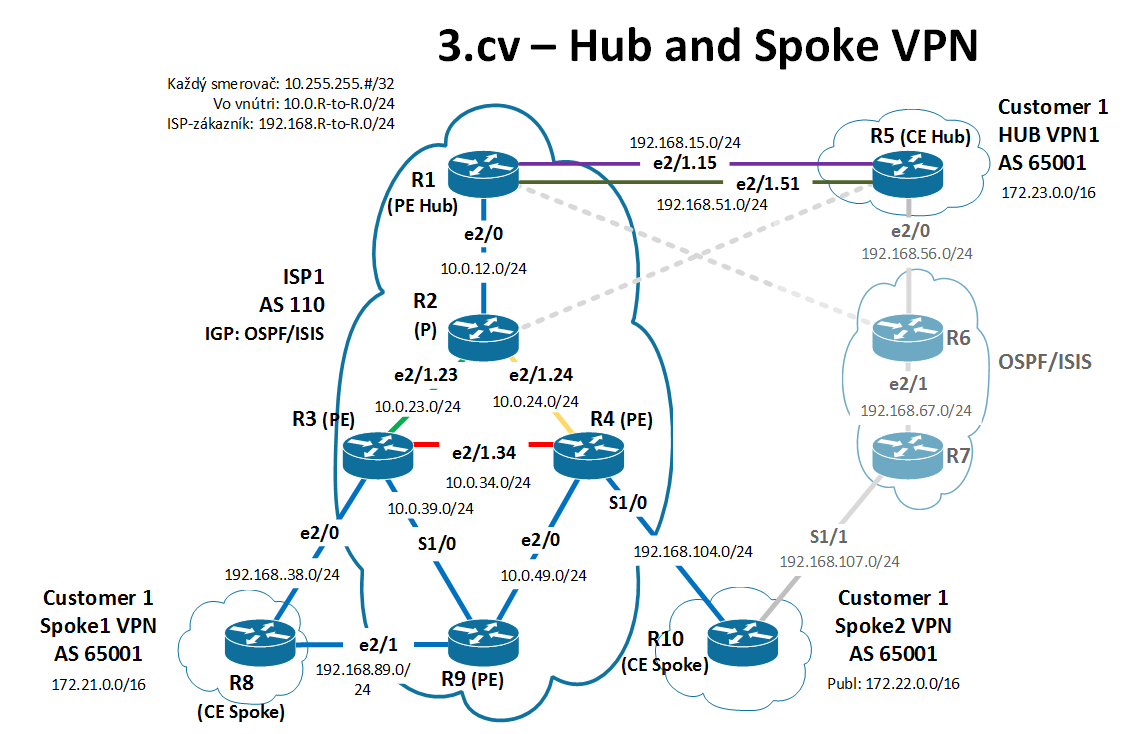
\includegraphics[width=14cm,keepaspectratio]{mpls_hub_spoke_topo}
\caption{Topológia MPLS Hub \& Spoke}
\label{fig:mpls_hub_spoke_topo}
\end{figure}

\begin{figure}[!htbp]
\centering
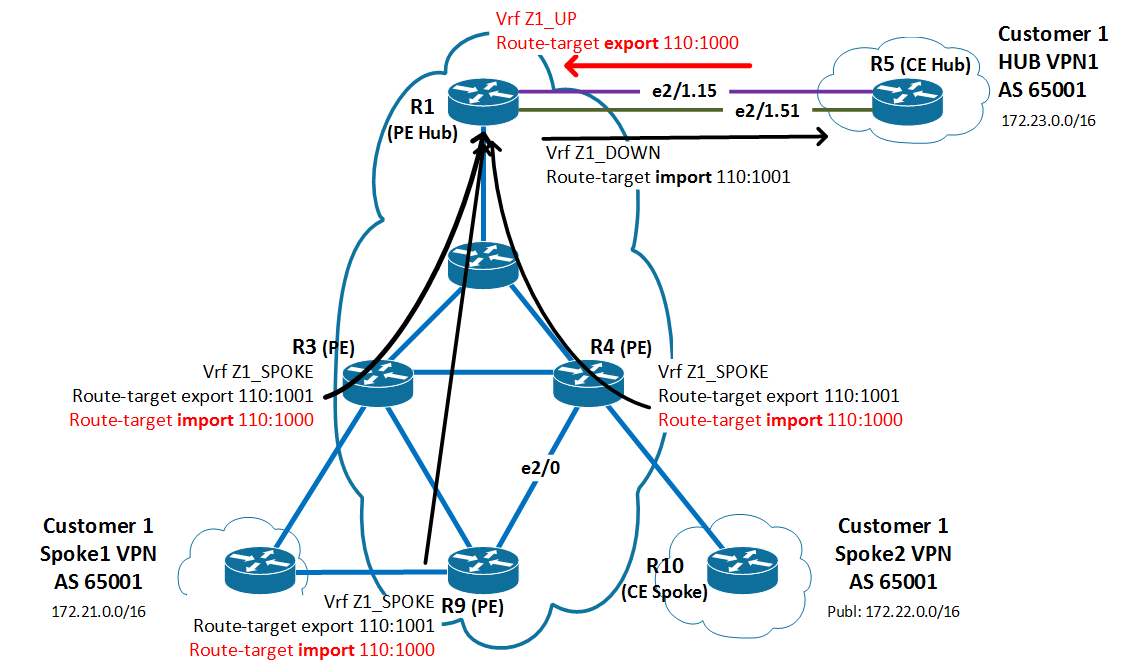
\includegraphics[width=14cm,keepaspectratio]{mpls_hub_spoke_route_target_topo}
\caption{Topológia MPLS Hub \& Spoke s Route Target}
\label{fig:mpls_hub_spoke_route_target_topo}
\end{figure}

\subsubsection{Konfigurácia}
\paragraph{}

\noindent
{\fontfamily{qcr}\selectfont
\begin{small}
\begin{alltt}
R5 (CE smerovač)
router bgp 65001
  address-family ipv4 unicast
    network 10.255.255.5 mask 255.255.255.255
    network 172.23.0.0 mask 255.255.255.0
    neighbor 192.168.15.1 activate
\end{alltt}
\end{small}
}

\paragraph{}
Pokračovali sme konfiguráciou 

\noindent
{\fontfamily{qcr}\selectfont
\begin{small}
\begin{alltt}
R1
no ip vrf RED

ip vrf Z1_DOWN
 rd 110:1001
 route-target import 110:1001

ip vrf Z1_UP
 rd 110:1000
 route-target export 110:1000

interface Ethernet2/1
 no ip address
 duplex half

interface Ethernet2/1.15
 encapsulation dot1Q 15
 ip vrf forwarding Z1_UP
 ip address 192.168.15.1 255.255.255.0

interface Ethernet2/1.51
 encapsulation dot1Q 51
 ip vrf forwarding Z1_DOWN
 ip address 192.168.51.1 255.255.255.0

router bgp 110
 address-family ipv4
  neighbor 10.255.255.3 activate
  neighbor 10.255.255.4 activate
  neighbor 10.255.255.9 activate
 exit-address-family
 
 address-family ipv4 vrf Z1_DOWN
  redistribute connected
  neighbor 192.168.51.5 remote-as 65001
  neighbor 192.168.51.5 activate
  neighbor 192.168.51.5 as-override
 exit-address-family
 
 address-family ipv4 vrf Z1_UP
  redistribute connected
  redistribute static
  neighbor 192.168.15.5 remote-as 65001
  neighbor 192.168.15.5 activate
  neighbor 192.168.15.5 as-override
  default-information originate
 exit-address-family

ip route vrf Z1_UP 0.0.0.0 0.0.0.0 192.168.15.5
mpls ldp router-id Loopback0
==============================================
R3#
!namiesto RED dal:
no ip vrf RED

int eth2/0
 ip addr 192.168.38.3

ip vrf Z1_SPOKE
 rd 110:1001
 route-target export 110:1001
 route-target import 110:1000

interface Ethernet2/0
 ip vrf forwarding Z1_SPOKE

router bgp 110
 address-family ipv4 vrf Z1_SPOKE
  redistribute connected
  neighbor 192.168.38.8 remote-as 65001
  neighbor 192.168.38.8 activate
  neighbor 192.168.38.8 as-override
 exit-address-family
=======================================
R4#sh run
!ip brf GREEN a RED zmazal a dal:

int s1/0
 ip addr 192.168.104.4 255.255.255.0

int e2/0
 ip addr 10.0.49.4 255.255.255.0

ip vrf Z1_SPOKE
 rd 110:1001
 route-target export 110:1001
 route-target import 110:1000

interface Serial1/0
 ip vrf forwarding Z1_SPOKE

router bgp 110
!namiesto RED a GREEN dal:

 address-family ipv4 vrf Z1_SPOKE
  redistribute connected
  neighbor 192.168.104.10 remote-as 65001
  neighbor 192.168.104.10 activate
  neighbor 192.168.104.10 as-override
 exit-address-family
=================================================
R9#
!ip vrf RED zmenil na:

ip vrf Z1_SPOKE
 rd 110:1001
 route-target export 110:1001
 route-target import 110:1000

interface Ethernet2/1
 ip addr 192.168.89.9 255.255.255.0
 ip vrf forwarding Z1_SPOKE

router bgp 110
!namiesto RED dal:

 address-family ipv4 vrf Z1_SPOKE
  redistribute connected
  neighbor 192.168.38.8 remote-as 65001
  neighbor 192.168.38.8 activate
  neighbor 192.168.38.8 as-override
 exit-address-family
============
R5

interface Ethernet2/1
 no ip address

interface Ethernet2/1.15
 encapsulation dot1Q 15
 ip address 192.168.15.5 255.255.255.0

interface Ethernet2/1.51
 encapsulation dot1Q 51
 ip address 192.168.51.5 255.255.255.0

router bgp 65001
 network 10.255.255.5 mask 255.255.255.255
 neighbor 192.168.51.1 remote-as 110
\end{alltt}
\end{small}
}

\paragraph{}
Parameter as-override zabezpečí, aby smerovače nezahadzovali siete, ktoré prechádzajú do rovnakého AS (65001). Príkaz redistribute connected distribuuje všetky pripojené siete zákazníka v rámci BGP. Tieto príkazy zadáme na smerovačoch R1 smerom k R5, na R9 k R8 a na R4 k R10.

\paragraph{}
Konfigurácia CE smerovačov je podobná, využíva však address-family, pretože zákazníci sa o VRF nezaujímajú. Na smerovačoch R5, R8 a R10 musíme zmeniť predošlú konfiguráciu BGP, teda pôvodné AS nahradíme AS 65001, ohlásime ich vlastné siete a aktivujeme spojenie na suseda.

\noindent
{\fontfamily{qcr}\selectfont
\begin{small}
\begin{alltt}
R5 (CE smerovač)
router bgp 65001
  address-family ipv4 unicast
    network 10.255.255.5 mask 255.255.255.255
    network 172.23.0.0 mask 255.255.255.0
    neighbor 192.168.15.1 activate
\end{alltt}
\end{small}
}

\subsubsection{Overenie}
\paragraph{}
Zadaním tohto príkazu sa presunie záznam z globálnej smerovacej tabuľky do smerovacej tabuľky vrf z1. Po zadaní príkazu je takisto potrebné na ňom nanovo zadať IP adresu. Overenie, že sa rozhranie pridalo do danej VRF, vykonáme príkazom \say{sh ip vrf}.

\noindent
{\fontfamily{qcr}\selectfont
\begin{small}
\begin{alltt}
R1#show ip vrf
TODO
\end{alltt}
\end{small}
}

\paragraph{}
Po správnej konfigurácii by sa na CE smerovačoch v BGP tabuľke pre ipv4 unicast mali objaviť všetky ohlasované siete smerovačov R5, R8 a R10 (Lo0 aj Lo1).

\noindent
{\fontfamily{qcr}\selectfont
\begin{small}
\begin{alltt}
R5#sh ip bgp ipv4 unicast
TODO
\end{alltt}
\end{small}
}

\paragraph{}
Rovnako sme použili Traceroute z R5 lo1 na R10 lo1

\noindent
{\fontfamily{qcr}\selectfont
\begin{small}
\begin{alltt}
R5#traceroute 172.22.0.1 source 172.23.0.1
TODO
\end{alltt}
\end{small}
}






\subsection{Draft Rosen}
\subsubsection{Popis}
\paragraph{}
Darth Vader je multicastová MPLS technológia. Pochádza z inej galaxie. Prvá zmienka bola v seriáli StarWars :)

\subsubsection{Konfigurácia}
\paragraph{}
Najprv zrusime vsetko, co sme nakonfigurovali pre hub and spoke. Potom:

\paragraph{}
r1 r5 treba vratit na jednu linku (zrusit trunky). 
\noindent
{\fontfamily{qcr}\selectfont
\begin{small}
\begin{alltt}
no int eth2/1.15
no int eth2/1.51
int eth2/1
ip addr 192.168.15.# 255.255.255.0
\end{alltt}
\end{small}
}



\paragraph{}
Najprv vymazeme VRFky z Hub \& Spoke
\noindent
{\fontfamily{qcr}\selectfont
\begin{small}
\begin{alltt}
!R1
no ip vrf Z1_DOWN
no ip vrf Z1_UP

!R3, R4, R9
no ip vrf Z1_SPOKE
\end{alltt}
\end{small}
}

\paragraph{}
Vytvorime novu VRFku pre klienta GREEN. Route target import a export bude rovnaky. Novu VRFku nastavime na R1, R3, R4 a R9.

\noindent
{\fontfamily{qcr}\selectfont
\begin{small}
\begin{alltt}
ip vrf GREEN
  rd 110:2
  route-target both 110:2
\end{alltt}
\end{small}
}

\paragraph{}
Aplikujeme VRFky na interfacey R1, R3, R4 a R9 a nanovo nahodime ipcky na interfejsoch:

\noindent
{\fontfamily{qcr}\selectfont
\begin{small}
\begin{alltt}
!R1
R1(config)#int eth2/1
R1(config-if)#ip vrf forwarding GREEN
% Interface Ethernet2/1 IPv4 disabled and address(es) removed due to enabling VRF GREEN
R1(config-if)#ip addr 192.168.15.1 255.255.255.0
R1(config-if)#no shut
R1(config-if)#exit
R1(config)#router bgp 110          
R1(config-router)#address-family ipv4 vrf GREEN
R1(config-router-af)#redistribute connected
R1(config-router-af)#neighbor 192.168.15.5 remote-as 65001
R1(config-router-af)#neighbor 192.168.15.5 activa         
*May 16 10:10:08.158: %BGP-5-ADJCHANGE: neighbor 192.168.15.5 vpn vrf GREEN Up 
R1(config-router-af)#neighbor 192.168.15.5 activate
R1(config-router-af)#neighbor 192.168.15.5 as-ov   
R1(config-router-af)#neighbor 192.168.15.5 as-override
\end{alltt}
\end{small}
}



KONFIGURACIA DRAFT ROSEN
mdt id pre zakaznika 239.10.10.10 - GREEN. v sieti zakaznika rozbehnut PIM sparse mode. RP bude R1, v sieti zakaznika to bude r5. konfigurujeme zakaznicke routre r8-r10. staticky join na r10 a pingat nanho.


Na vsetkych routroch:
\noindent
{\fontfamily{qcr}\selectfont
\begin{small}
\begin{alltt}
ip multicast-routing
\end{alltt}
\end{small}
}




Na PE routroch 1,3,4,9

\noindent
{\fontfamily{qcr}\selectfont
\begin{small}
\begin{alltt}
ip multicast-routing vrf GREEN
\end{alltt}
\end{small}
}




Na providerskych routroch zadat pre vsetky interfejsy (aj na loopback0) prikaz

\noindent
{\fontfamily{qcr}\selectfont
\begin{small}
\begin{alltt}
ip pim sparse-mode
\end{alltt}
\end{small}
}

aby sme zapli PIM Sparse Mode, kvoli sireniu multicastov. V trojuholniku staci davat prikaz iba na subinterfejsy. Rovnako urobime aj na CE routroch, ale iba pre interfejsy smerujuce na PE routre.






Nastavime RP pre providera na R1 a pre zakaznika na R5.\\
PE routre
\noindent
{\fontfamily{qcr}\selectfont
\begin{small}
\begin{alltt}
ip pim rp-address 10.255.255.1
\end{alltt}
\end{small}
}

Zakaznicke CE routre
\noindent
{\fontfamily{qcr}\selectfont
\begin{small}
\begin{alltt}
ip pim rp-address 172.23.0.1
\end{alltt}
\end{small}
}



Na PE routroch pouzijeme prikazy

\noindent
{\fontfamily{qcr}\selectfont
\begin{small}
\begin{alltt}
ip vrf GREEN
  mdt default 239.10.10.10
\end{alltt}
\end{small}
}

Tak ho priradime do multicastovej skupiny.






Na PE routroch musime nastavit zakaznicky RP pre VRF GREEN.

\noindent
{\fontfamily{qcr}\selectfont
\begin{small}
\begin{alltt}
R9(config)#ip pim vrf GREEN rp-address 172.23.0.1
\end{alltt}
\end{small}
}



Na CE routroch priradime loopback do multicastovej skupiny

\noindent
{\fontfamily{qcr}\selectfont
\begin{small}
\begin{alltt}
int lo0
  ip igmp join-group 239.10.10.10
\end{alltt}
\end{small}
}





\subsubsection{Overenie − Zakladná MP−BGP konektivita}
\paragraph{}
\noindent
{\fontfamily{qcr}\selectfont
\begin{small}
\begin{alltt}
show ip route vrf GREEN
show ip vrf
\end{alltt}
\end{small}
}


\noindent
{\fontfamily{qcr}\selectfont
\begin{small}
\begin{alltt}
R4(config-router-af)#do sh ip route vrf GREEN

Routing Table: GREEN
...

Gateway of last resort is not set

      10.0.0.0/32 is subnetted, 3 subnets
B        10.255.255.5 [200/0] via 10.255.255.1, 00:08:23
B        10.255.255.8 [200/0] via 10.255.255.3, 00:03:21
B        10.255.255.10 [20/0] via 192.168.104.10, 00:00:23
B     172.21.0.0/16 [200/0] via 10.255.255.3, 00:03:21
B     172.22.0.0/16 [20/0] via 192.168.104.10, 00:00:23
B     172.23.0.0/16 [200/0] via 10.255.255.1, 00:08:23
B     192.168.15.0/24 [200/0] via 10.255.255.1, 00:08:53
B     192.168.38.0/24 [200/0] via 10.255.255.3, 00:04:05
B     192.168.56.0/24 [200/0] via 10.255.255.1, 00:08:23
B     192.168.89.0/24 [200/0] via 10.255.255.3, 00:03:21
      192.168.104.0/24 is variably subnetted, 2 subnets, 2 masks
C        192.168.104.0/24 is directly connected, Serial1/0
L        192.168.104.4/32 is directly connected, Serial1/0
B     192.168.107.0/24 [20/0] via 192.168.104.10, 00:00:23





R8#show ip bgp ipv4 unicast 
BGP table version is 42, local router ID is 10.255.255.8
Status codes: s suppressed, d damped, h history, * valid, > best, i - internal, 
              r RIB-failure, S Stale, m multipath, b backup-path, f RT-Filter, 
              x best-external, a additional-path, c RIB-compressed, 
Origin codes: i - IGP, e - EGP, ? - incomplete
RPKI validation codes: V valid, I invalid, N Not found

     Network          Next Hop            Metric LocPrf Weight Path
 *   10.255.255.5/32  192.168.89.9                           0 110 110 i
 *>                   192.168.38.3                           0 110 110 i
 *>  10.255.255.8/32  0.0.0.0                  0         32768 ?
 *   10.255.255.10/32 192.168.89.9                           0 110 110 ?
 *>                   192.168.38.3                           0 110 110 ?
 *>  172.21.0.0       0.0.0.0                  0         32768 i
 *   172.22.0.0       192.168.89.9                           0 110 110 i
 *>                   192.168.38.3                           0 110 110 i
 *   172.23.0.0       192.168.89.9                           0 110 110 i
 *>                   192.168.38.3                           0 110 110 i
 *   192.168.15.0     192.168.89.9                           0 110 ?
 *>                   192.168.38.3                           0 110 ?
 *   192.168.38.0     192.168.89.9                           0 110 ?
 *                    192.168.38.3             0             0 110 ?
     Network          Next Hop            Metric LocPrf Weight Path
 *>                   0.0.0.0                  0         32768 ?
 *   192.168.56.0     192.168.89.9                           0 110 110 ?
 *>                   192.168.38.3                           0 110 110 ?
 *   192.168.89.0     192.168.89.9             0             0 110 ?
 *                    192.168.38.3                           0 110 ?
 *>                   0.0.0.0                  0         32768 ?
 *   192.168.104.0    192.168.89.9                           0 110 ?
 *>                   192.168.38.3                           0 110 ?
 *   192.168.107.0    192.168.89.9                           0 110 110 ?
 *>                   192.168.38.3                           0 110 110 ?







R8#ping 172.22.0.1 source 172.21.0.1
Type escape sequence to abort.
Sending 5, 100-byte ICMP Echos to 172.22.0.1, timeout is 2 seconds:
Packet sent with a source address of 172.21.0.1 
!!!!!
Success rate is 100 percent (5/5), round-trip min/avg/max = 52/56/60 ms





R4(config-router-af)#do ping vrf GREEN 172.23.0.1
Type escape sequence to abort.
Sending 5, 100-byte ICMP Echos to 172.23.0.1, timeout is 2 seconds:
!!!!!
Success rate is 100 percent (5/5), round-trip min/avg/max = 52/59/72 ms

\end{alltt}
\end{small}
}

============\\
OVERENIE Multicastovych tunelov\\
==============\\
\noindent
{\fontfamily{qcr}\selectfont
\begin{small}
\begin{alltt}
R1(config)#ip pim rp-address 10.255.255.1
R1(config)#
*May 16 10:59:35.306: %LINEPROTO-5-UPDOWN: Line protocol on Interface Tunnel0, changed state to up
*May 16 10:59:35.474: %LINEPROTO-5-UPDOWN: Line protocol on Interface Tunnel1, changed state to up
\end{alltt}
\end{small}
}



\paragraph{}
MPLS funguje, Draft Rosen nefunguje.


\end{document}